\documentclass{beamer}
\usepackage[utf8]{inputenc}

\usetheme{Madrid}
\usecolortheme{default}
\usepackage{amsmath,amssymb,amsfonts,amsthm}
\usepackage{txfonts}
\usepackage{tkz-euclide}
\usepackage{listings}
\usepackage{adjustbox}
\usepackage{array}
\usepackage{tabularx}
\usepackage{gvv}
\usepackage{lmodern}
\usepackage{circuitikz}
\usepackage{tikz}
\usepackage{graphicx}
\usepackage{caption}
\captionsetup{labelformat=empty}  % removes "Figure:"


\setbeamertemplate{page number in head/foot}[totalframenumber]

\usepackage{tcolorbox}
\tcbuselibrary{minted,breakable,xparse,skins}



\definecolor{bg}{gray}{0.95}
\DeclareTCBListing{mintedbox}{O{}m!O{}}{%
	breakable=true,
	listing engine=minted,
	listing only,
	minted language=#2,
	minted style=default,
	minted options={%
		linenos,
		gobble=0,
		breaklines=true,
		breakafter=,,
		fontsize=\small,
		numbersep=8pt,
		#1},
	boxsep=0pt,
	left skip=0pt,
	right skip=0pt,
	left=25pt,
	right=0pt,
	top=3pt,
	bottom=3pt,
	arc=5pt,
	leftrule=0pt,
	rightrule=0pt,
	bottomrule=2pt,
	toprule=2pt,
	colback=bg,
	colframe=orange!70,
	enhanced,
	overlay={%
		\begin{tcbclipinterior}
			\fill[orange!20!white] (frame.south west) rectangle ([xshift=20pt]frame.north west);
	\end{tcbclipinterior}},
	#3,
}
\lstset{
	language=C,
	basicstyle=\ttfamily\small,
	keywordstyle=\color{blue},
	stringstyle=\color{orange},
	commentstyle=\color{green!60!black},
	numbers=left,
	numberstyle=\tiny\color{gray},
	breaklines=true,
	showstringspaces=false,
}
\begin{document}

\title 
{2.10.73}
\date{October 1,2025}

\author 
{Navya Priya - EE25BTECH11045}
\graphicspath{./figs}

\frame{\titlepage}
\begin{frame}{Question}
  Let $\vec{A}$, $\vec{B}$ and $\vec{C}$ be unit vectors. Suppose that  $\vec{A}\cdot\vec{B}$ =  $\vec{A}\cdot\vec{C}$= 0, and that the angle between  $\vec{B}$ and  $\vec{C}$ is $\frac{\pi}{6}$. Then $\vec{A}= \pm2(\vec{B}\times\vec{C})$
\end{frame}

\begin{frame}{Theoretical Solution}
 Let us solve the given equation theoretically and then verify the solution computationally.\\

Since $\vec{A}\cdot\vec{B}$ =  $\vec{A}\cdot\vec{C}$= 0, it follows that $\vec{A}$ is perpendicular to both $\vec{B}$ and $\vec{C}$. Therefore A is parallel(or anti-parallel) to the cross product of $\vec{B}$ and $\vec{C}$.

\begin{align}
    \vec{A}\,=\,\lambda(\vec{B}\times\vec{C})
\end{align}
From the given question,
\begin{align}
    \vec{B}^\top\vec{C}=\text{cos}\brak{\frac{\pi}{6}}
\end{align}
We know that,
\begin{align}
 \brak{\vec{B}^\top\vec{C}}^{2}\,+\,||\vec{B}\times\vec{C}||^{2}=||\vec{B}||^{2}||\vec{C}||^{2}
\end{align}
\end{frame}

\begin{frame}{Theoretical Solution}
 \begin{align}
 \implies   ||\vec{B}\times\vec{C}||^{2}\,=\,\frac{1}{4}
\end{align}
\begin{align}
   \implies   ||\vec{B}\times\vec{C}||\,=\,\frac{1}{2}
\end{align}
As $\vec{A}$ is a unit vector,\\
from(1)
\begin{align}
    ||\vec{A}||\,=\,||\lambda(\vec{B}\times\vec{C})||
\end{align}
\begin{align}
    1\,=\,|\lambda|\frac{1}{2}
\end{align}
Hence
\begin{align}
 \lambda\,=\,\pm 2
\end{align}
\begin{align}
    \therefore \vec{A}\,=\,\pm 2(\vec{B}\times\vec{C})
\end{align}
\end{frame}

\begin{frame}[fragile]{C code}
\begin{lstlisting}
#include <stdio.h>
#include <math.h>

int main() {
    // Define B and C as given
    double B[3] = {0.5, sqrt(3)/2, 0};
    double C[3] = {0.5, -sqrt(3)/2, 0};
    double cross[3], A1[3], A2[3];

    // Cross product B x C
    cross[0] = B[1]*C[2] - B[2]*C[1];
    cross[1] = B[2]*C[0] - B[0]*C[2];
    cross[2] = B[0]*C[1] - B[1]*C[0];

    // A = ±2(B x C)
    for (int i=0; i<3; i++) {
        A1[i] = 2 * cross[i];
        A2[i] = -2 * cross[i];
    }
\end{lstlisting}
\end{frame}

\begin{frame}[fragile]{C code}
\begin{lstlisting}
    // Print results
    printf("Vector B = (%.2f, %.2f, %.2f)\n", B[0], B[1], B[2]);
    printf("Vector C = (%.2f, %.2f, %.2f)\n", C[0], C[1], C[2]);
    printf("Cross Product (B x C) = (%.2f, %.2f, %.2f)\n", cross[0], cross[1], cross[2]);
    printf("A1 = +2(B x C) = (%.2f, %.2f, %.2f)\n", A1[0], A1[1], A1[2]);
    printf("A2 = -2(B x C) = (%.2f, %.2f, %.2f)\n", A2[0], A2[1], A2[2]);

    return 0;
}
\end{lstlisting}
\end{frame}

\begin{frame}[fragile]{CallC.py}
\begin{lstlisting}
import ctypes
import numpy as np
import matplotlib.pyplot as plt

# Load shared library
lib = ctypes.CDLL("./vectors.so")   # use "vectors.dll" on Windows

# Define argument and return types
lib.compute_vectors.argtypes = [
    np.ctypeslib.ndpointer(dtype=np.float64, ndim=1, flags="C_CONTIGUOUS"),
    np.ctypeslib.ndpointer(dtype=np.float64, ndim=1, flags="C_CONTIGUOUS"),
    np.ctypeslib.ndpointer(dtype=np.float64, ndim=1, flags="C_CONTIGUOUS"),
    np.ctypeslib.ndpointer(dtype=np.float64, ndim=1, flags="C_CONTIGUOUS"),
]
lib.compute_vectors.restype = None

\end{lstlisting}
\end{frame}

\begin{frame}[fragile]{CallC.py}
\begin{lstlisting}

# Input vectors
B = np.array([0.5, np.sqrt(3)/2, 0.0], dtype=np.float64)
C = np.array([0.5, -np.sqrt(3)/2, 0.0], dtype=np.float64)

# Output arrays
A1 = np.zeros(3, dtype=np.float64)
A2 = np.zeros(3, dtype=np.float64)

# Call C function
lib.compute_vectors(B, C, A1, A2)

# --- Plot ---
fig = plt.figure()
ax = fig.add_subplot(111, projection="3d")
\end{lstlisting}
\end{frame}

\begin{frame}[fragile]{CallC.py}
\begin{lstlisting}
vectors = {"B": B, "C": C, "A1": A1, "A2": A2}
colors = {"B": "r", "C": "g", "A1": "b", "A2": "m"}

for name, vec in vectors.items():
    ax.quiver(0,0,0, vec[0], vec[1], vec[2], color=colors[name], label=name)
    ax.text(vec[0], vec[1], vec[2], f"{name}{tuple(vec.round(2))}")

ax.set_xlabel("X")
ax.set_ylabel("Y")
ax.set_zlabel("Z")
ax.set_title("Vectors from C + Python (ctypes)")
ax.legend()
plt.show()

\end{lstlisting}
\end{frame}

\begin{frame}[fragile]{Plot.py}
\begin{lstlisting}
import numpy as np
import matplotlib.pyplot as plt
from mpl_toolkits.mplot3d import Axes3D

# Define vectors
B = np.array([1, 0, 0])
C = np.array([np.cos(np.pi/6), np.sin(np.pi/6), 0])
cross_BC = np.cross(B, C)
A1 = 2 * cross_BC
A2 = -2 * cross_BC

# Plotting
fig = plt.figure()
ax = fig.add_subplot(111, projection='3d')

# Function to draw vectors
def draw_vector(ax, vec, color, label):
    ax.quiver(0, 0, 0, vec[0], vec[1], vec[2], color=color, label=label)
\end{lstlisting}
\end{frame}

\begin{frame}[fragile]{Plot.py}
\begin{lstlisting}
# Draw vectors
draw_vector(ax, B, 'r', 'B')
draw_vector(ax, C, 'g', 'C')
draw_vector(ax, A1, 'b', 'A = +2(B×C)')
draw_vector(ax, A2, 'm', 'A = -2(B×C)')

# Axes settings
ax.set_xlim([-2, 2])
ax.set_ylim([-2, 2])
ax.set_zlim([-2, 2])
ax.set_xlabel('X')
ax.set_ylabel('Y')
ax.set_zlabel('Z')
ax.legend()
ax.set_title("Vectors A, B, C in 3D")

plt.show()

\end{lstlisting}
\end{frame}

\begin{frame}{Plot}
  To verify the solution computationally let us assume the vectors $\vec{B}$ and $\vec{C}$ as 

\centering
$\vec{B}=\myvec{1\\0\\0}$ and $\vec{C}=\myvec{\frac{\sqrt{3}}{2}\\[4pt]\frac{1}{2}\\0}$  
\end{frame}

\begin{frame}{Plot}
    \begin{figure}[H]
\centering
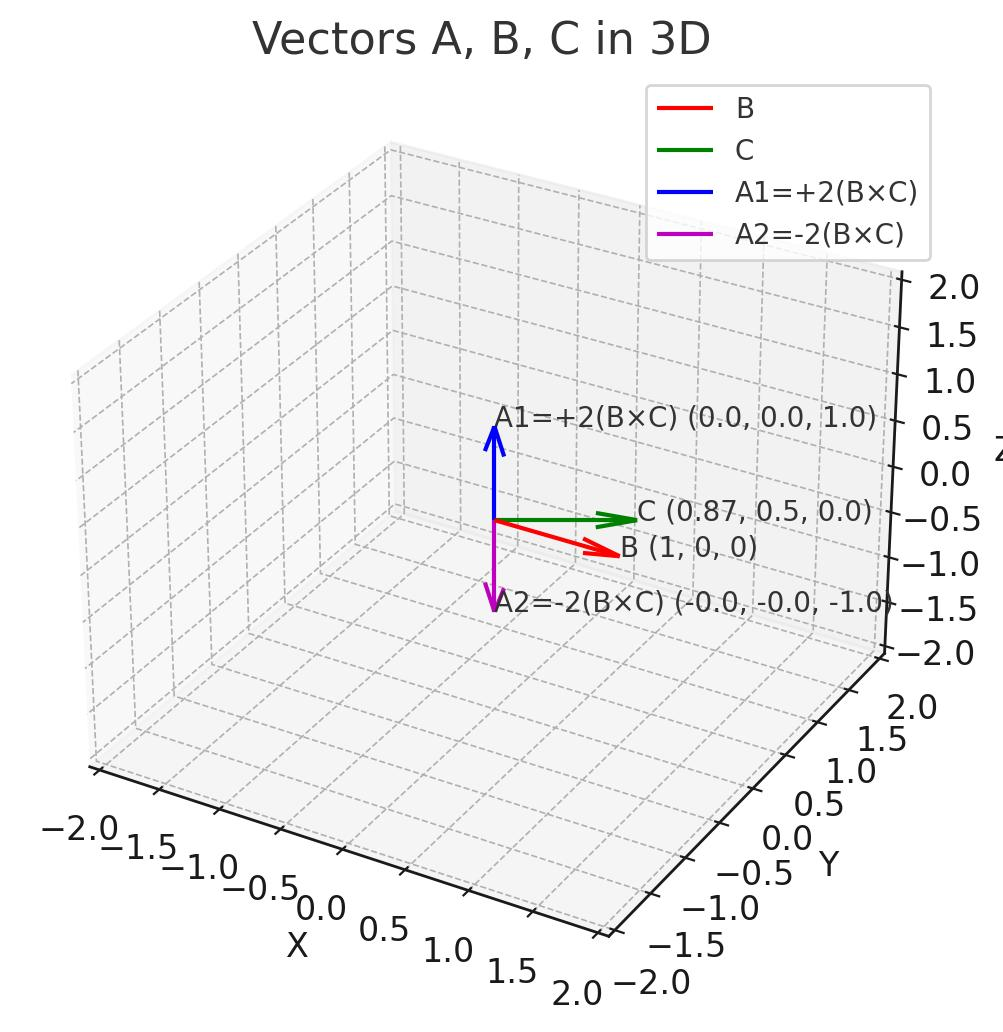
\includegraphics[width=0.5\columnwidth]{figs/graph.png}
\label{fig:graph.png}
\end{figure}
\end{frame}












\end{document}